\documentclass[a4paper, 11pt]{article}

\usepackage{graphicx}


\usepackage{wrapfig}
\usepackage{lipsum}

\usepackage[utf8]{inputenc}

\usepackage{mathpazo} % Use the Palatino font
\usepackage[T1]{fontenc} % Required for accented characters
\linespread{1.05} % Change line spacing here, Palatino benefits from a slight increase by default

\usepackage{float}
\usepackage{hyperref}
\hypersetup{
	colorlinks=true, 		% Aktivieren von farbigen Links im Dokument
	linkcolor=blue, 	% Farbe festlegen
	urlcolor=blue,
	linktocpage=true, 		% Nicht der Text sondern die Seitenzahlen in Verzeichnissen klickbar
	bookmarksnumbered=true 	% Überschriftsnummerierung im PDF Inhalt anzeigen.
}
\usepackage[ngerman]{babel}
\usepackage{tabularx}
\usepackage[table,xcdraw]{xcolor}
\usepackage{listings}
\usepackage{color}
 
\definecolor{pblue}{rgb}{0.13,0.13,1}
\definecolor{pgreen}{rgb}{0,0.5,0}
\definecolor{pred}{rgb}{0.9,0,0}
\definecolor{pgrey}{rgb}{0.46,0.45,0.48}

\usepackage{listings}
\lstset{language=Java,
  showspaces=false,
  showtabs=false,
  breaklines=true,
  showstringspaces=false,
  breakatwhitespace=true,
  commentstyle=\color{pgreen},
  keywordstyle=\color{pblue},
  stringstyle=\color{pred},
  basicstyle=\ttfamily,
  moredelim=[il][\textcolor{pgrey}]{$$},
  moredelim=[is][\textcolor{pgrey}]{\%\%}{\%\%}
}

\makeatletter

\renewcommand{\maketitle}{ % Customize the title - do not edit title and author name here, see the TITLE block below
\begin{flushright} % Right align
{\LARGE\@title} % Increase the font size of the title

\vspace{10pt} % Some vertical space between the title and author name

{\large\@author} % Author name
\\\@date % Date

\vspace{20pt} % Some vertical space between the author block and abstract
\end{flushright}
}

\title{\textbf{Arbeitsdokumentation des Backendteam}} 

\author{Team Backend} 

\date{\today} % Date

\begin{document}
\renewcommand{\@listI}{\itemsep=0pt} % Reduce the space between items in the itemize and enumerate environments and the bibliography

\maketitle % Print the title section

Die Umsetzung der in der API-Spec definierten Funktionalität erfolgt im
Backend. Dies ist eine Java-Applikation, welche auf einem
Tomcat-Appli\-ka\-tions\-server läuft. Die Applikation übernimmt unter anderem
folgende Aufgaben:

\begin{itemize}
    \item Bereitstellen der Routen
    \item Businesslogik
    \item Authentifizierung und Authorisierung
    \item Speichern in einer Datenbank
\end{itemize}

\section{Einstieg in Spring Boot}

Die Entwicklung erfolgt mithilfe des Frameworks
\href{https://en.wikipedia.org/wiki/Spring_Boot#Spring_Boot}{Spring Boot}. Das
Framework bietet verschiedene Features, die die Entwicklung erleichtern oder
strkturieren. Es ist zum Beispiel möglich, einen
\href{https://de.wikipedia.org/wiki/Objektrelationale_Abbildung}{objektrelationalen
Mapper}
zu nutzen, der den Datenbankzugriff stark abstrahiert. Auch das Bereitstellen
des Web-Services wird durch Spring Boot vereinfacht. Zusätzlich hat das
Framework eine gewissen \emph{Meinung}, mit welchen Mustern entwickelt werden
soll.

Zum Einstieg in das Backend-Projekt betrachten wir die Flugzeugverwaltung. Die
findet im Paket \texttt{Plane} statt, in dem zwei Klassen und ein Interface
definiert werden (vgl. Abbildung \ref{fig:planes_package}).

\begin{figure}[htpb]
    \centering
    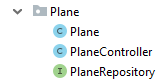
\includegraphics{images/plane_package.png}
    \caption{Inhalt des Package \texttt{Plane}}
    \label{fig:planes_package}
\end{figure}

Dabei ist die Klasse \texttt{Plane} das Business-Objekt, welches ein Flugzeug
repräsentiert. Im \texttt{PlaneController} werden die Webservice-Routen und die
Business-Logik definiert und das \texttt{PlaneRepository} abstrahiert das
Speichern von \texttt{Plane}-Objekten in der Datenbank.

Schauen wir uns nun zunächst einen Ausschnitt aus der \texttt{Plane}-Klasse an:

\begin{lstlisting}
@Entity
public class Plane {

    @Id
    @GeneratedValue(strategy = GenerationType.IDENTITY)
    private Integer id;
    private String number;
    private String name;
    ...
}
\end{lstlisting}

Die \lstinline{@Entity}-Annotation gibt an, dass die Klasse in der Datenbank
gespeichert werden soll, wobei die \lstinline{id} der Primärschlüssel hierfür
ist und vom Framework generiert werden soll.

\begin{figure}[htpb]
    \centering
    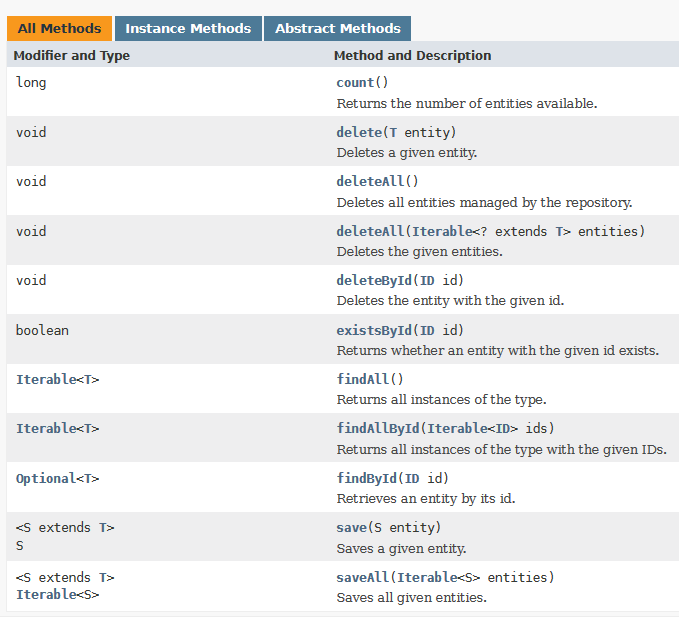
\includegraphics[width=\textwidth]{images/crudrepository.png}
    \caption{Ausschnitt der Methoden, die das PlaneRepository bereitstellt}
    \label{fig:crudrepository}
\end{figure}

Das \texttt{PlaneRepository} verwaltet dann die Datenbank-Interaktion und
stellt dafür unter anderem die Methoden aus Abbildung \ref{fig:crudrepository}
bereit. Diese Methoden erbt es von einem Interface, welches aus dem
Spring-Framework kommt. Daher wird der Datenbankzugriff in der Entwicklung
stark vereinfacht. Es ist an keiner Stelle nötig, SQL-Befehle zu formulieren.
Auch Schemata werden automatisch generiert. Dies ist ein besonders großer
Vorteil, da so eine Änderung in der Java-Klasse automatisch im Datenbankschema
übernommen wird. 

\begin{figure}[htpb]
    \centering
    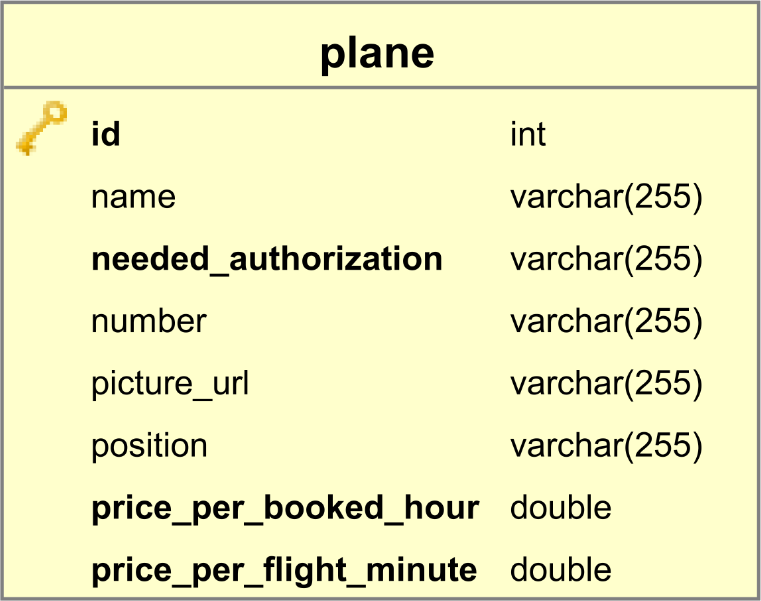
\includegraphics[width=0.4\textwidth]{images/erm/plane.png}
    \caption{Generierte Tabelle, die \texttt{Plane}-Objekte speichert}
    \label{fig:plane_table}
\end{figure}

Abbildung \ref{fig:plane_table} zeigt die MySQL-Tabelle, die vom
objekt-relationalen Mapper generiert wurde, um die \texttt{Plane}-Objekte zu
persitieren. Diese Tabelle wird automatisch durch die Entity-Annotation
erstellt. Wenn sich die Klasse verändert, wird auch beim nächsten Start der
Applikation auch die Tabelle geändert. Durch diese Abstraktion wird ein
hypothetisches Datenbank-Team in der Entwicklung unnötig, da nur noch zu
Kontroll- und Test-Zwecken direkt auf die Datenbank zugegriffen wird.

Der \texttt{PlaneController} enthält nun die Business-Logik:

\begin{lstlisting}
@RestController
@RequestMapping(path = "planes")
public class PlaneController {
...
    @GetMapping(path = "/{id}")
    public Plane detail(@PathVariable int id) {

    return planeRepository.findById(id)
            .orElseThrow(() -> new NoSuchElementException();
    }
...
}
\end{lstlisting}

Hier ist die Definition der unter dem Pfad \url{<server>:<port>/planes/{id}}
anzufindengen Methode gezeigt. Es wird in der URL also Parameter angegeben,
welches Flugzeug angezeigt werden soll, woraufhin das Flugzeug in der Datenbank
gesucht wird. Wird es gefunden, wird es zurückgegeben, wird kein Flugzeug
gefunden, wird eine \lstinline{Exception} geworfen. Hierbei übernimmt Spring
Boot, oder genauer, die Jackson-Bibliothek das \emph{Marshalling} und
\emph{Unmarshalling}, also das Umwandeln von JSON zu einfachen Java-Objekten
und umgekehrt. Außerdem gibt es eine Klasse, welche Exceptions fängt und
daraufhin an den Client passende Fehlermeldungen zurücksendet.

Dieser Dreiklang aus Business-Objekt, dazugehörigem Controller und Repository
ist relativ typisch für das Projekt.

\section{Die Business-Objekte und -Logik}

Eine Übersicht über die Business-Objekte des Projekts kann das Diagramm in
Abbildung \ref{fig:erm_all} geben. Es ist dabei zu beachten, dass alle diese
Tabellen vom objekt-relationalen Mapper generiert wurden. Assoziationen werden
im Quellcode über Annotationen wie \lstinline{@OneToOne},
\lstinline{@OneToManty} und \lstinline{@ManyToMany} zwischen den Objekten
hergestellt.

\begin{figure}[htpb]
    \centering
    \includegraphics[width=\textwidth]{images/erm/all_orthogonal.png}
    \caption{Diagramm des Datenbanktabellen}
    \label{fig:erm_all}
\end{figure}

\subsection{Member}

% grober Aufbau

% Herausforderung: Offices

\subsection{Transactions}

% Entscheidung für jeweils zwei parallele Transaxtionen statt
% "Geld geht von (a) nach (b)" / _geschlossenes System_

\subsection{VereinsAccount}

\subsection{Events}

% Transactions

% Email
%% async
%% Schwäche: Nicht gesendete Mails _unsichtbar_

\subsection{ExceptionHandling}

\section{Security}

\subsection{Authentifizierung}

\subsection{Authorisierung}

\end{document}
